\section{Datenbankmodelle}
\label{datenmodelle}
In diesem Abschnitt werden die Grundlagen des Graph-basierten Datenbankmodells  skizziert. Dieses Graphmodell ist im Rahmen dieser Arbeit von wesentlicher Bedeutung. Schließlich vereint die in \autoref{chap:db2graph} beschriebene Graph-Erweiterung, Elemente des relationalen und Graph-basierten Datenbankmodells. Grundkenntnisse über das relationalen Modell werden dabei hingegen im Rahmen dieser Arbeit vorausgesetzt. Sollten keine Grundkenntnisse über relationale Datenbanksysteme vorhanden sein, empfehlen sich \cite{rdbms_book} und \cite{codd_relational_model} als Einstieg.

Um die Grundlagen des Graphmodells in diesem Abschnitt zu vermittelten, werden die folgenden Aspekte des Modells angesprochen:
\begin{itemize}
    \item Herkunft und Verbreitung,
    \item Struktur und Schema.
\end{itemize}
Die Beschränkung auf diese Aspekte wurde dabei vorgenommen, da die Erläuterung weiterer Aspekt über den Rahmen dieser Arbeit hinausgehen würde. 

Anschließend findet eine kurze Gegenüberstellung des Graphmodells mit dem relationalen Modell statt. Im nächsten Unterabschnitt wird auf die Abfragesprachen von relationalen und Graphdatenbanksystemen eingegangen.

Zum Schluss werden die Informationen nochmals kurz zusammengefasst. 

\subsection{Herkunft und Verbreitung}
Das Graphmodell als Datenbankmodell hat seinen Ursprung in der heutigen Form im Jahr 1999 \cite{gdbms}. Dabei wurde das Graphmodell mit der Motivation entwickelt, vermeintliche Nachteile oder Probleme des relational Modells auszuräumen \cite{gdbms}.

Graphdatenbanksysteme und das Graphmodell sind heute als vergleichbar junge Technologien noch nicht so weit verbreitet wie beispielsweise, dass relationale Modell. Mit 1,7 \% Marktanteil ordnen sich Graphdatenbanksysteme noch weit hinter anderen Technologien ein, wie \textit{Document Stores}, \textit{Key-Values Stores} oder \textit{Wide column stores} \cite{db_engines_ranking_july} (\autoref{fig:dbms_marketshare}). Jedoch haben Graphdatenbanksysteme seit 2013 einen erheblichen Aufschwung in ihrer Popularität erfahren \cite{db_engines_ranking_july}. Der dort ermittelte Popularitäts-Score für die verschiedenen Datenbankkategorien zeigt dabei hierbei einen klaren Aufwärtstrend \cite{db_engines_ranking_july}. 

\begin{figure}[ht]
    \centering
    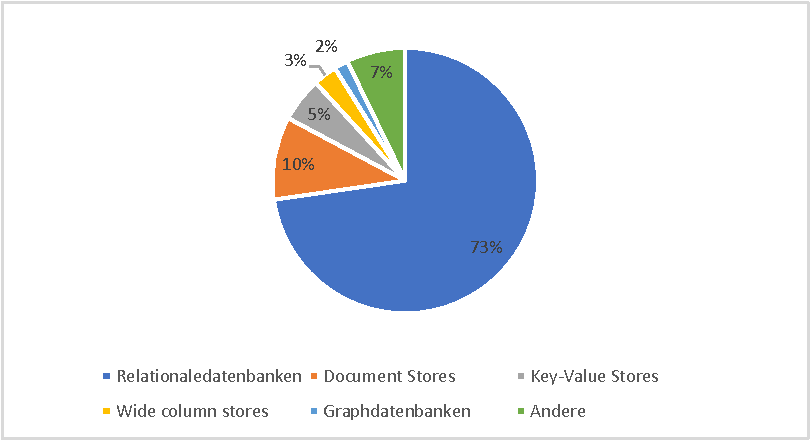
\includegraphics[width=\textwidth]{images/marketshare_dbms.pdf}
    \caption{Marktanteile nach Datenbankmanagementsystem-Kategorie}
    \label{fig:dbms_marketshare}
    \vspace{1em}
    \textit{Bei den hier abgebildeten Werten handelt es sich um die aufgerundeten Werte aus} \cite{db_engines_ranking_july}\textit{.}
\end{figure}

\subsection{Struktur und Schema}
\label{datenmodelle:structure}
Die Grundlage des Graphmodells stellen sogenannte Knoten und Kanten dar (\textit{engl. Vertexes oder Vertices}) und Kanten (\textit{engl. Edges}) dar. Diese Knoten und Kanten bilden dabei zusammen einen sogenannten Graphen. So werden in einem Graphen einerseits Entitäten in Form eines Knotens repräsentiert \cite{gdbms}, wie beispielsweise \textit{Robin} oder \textit{ID3} in \autoref{fig:beispiel_graph}. Anderseits bildet es auch explizit Beziehungen zwischen Entitäten mittels Kanten ab \cite{gdbms}, wie \textit{besitzt}, \textit{besaß} oder \textit{kennt} in \autoref{fig:beispiel_graph}. Auf Beziehungen wird in \autoref{datenmodelle:beziehungen} weiter eingegangen. 

Knoten und Kanten können dabei in diesem Modell anhand von sogenannten Labels organisiert werden. So können Knoten oder Kanten, die eine ähnliche Rolle einnehmen, dieselben Labels zugewiesen werden. Die Verwendung von Labels wird hierbei in \autoref{fig:beispiel_graph} durch die unterschiedlichen Farben gekennzeichnet. So werden darin die als Auto gelabelten Knoten in hellbraun markiert, während die Personen rot eingefärbt werden. Sie sind in ihrer Funktion allerdings nicht mit Tabellen aus dem relationalen Modell vergleichbar. Dies liegt darin begründet, dass Entitäten mit einem bestimmten Label unterschiedliche Informationen aufweisen können. So werden bei \autoref{fig:beispiel_graph} alle Personen-Knoten mit ihrer \texttt{Name}-Property abgebildet, während alle Auto-Knoten ihre \texttt{Modell}-Property darin aufführen.

Das Graphmodell setzt, anders als das relationale Modell, auf ein flexibles Datenbankschema \cite{gdbms}. Durch dieses flexible Schema fällt es leicht heterogene Daten in dem Graphmodell abzubilden. 

\begin{figure}[ht]
    \centering
    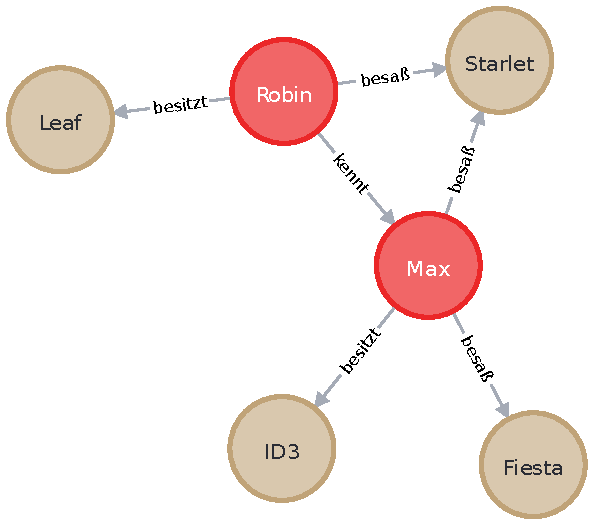
\includegraphics[width=0.75\textwidth]{images/example_graph.pdf}
    \caption{Beispiel Graph}
    \vspace{1em}
    \textit{Hier wird ein Beispiel Graph abgebildet der die Besitzbeziehungen zwischen einer Person (Besitzer) und einem Auto modelliert.}
    \label{fig:beispiel_graph}
\end{figure}

\subsection{Beziehungen}
\label{datenmodelle:beziehungen}
Beim Graphmodell stellen Beziehungen eine grundlegende Struktur in einem Graphen dar \cite{gdbms}, siehe \autoref{datenmodelle:structure}. Dabei werden im Graphmodell Beziehungen direkt zwischen Entitäten aufgebaut \cite{gdbms}, wie in \autoref{fig:beispiel_graph} erkennbar. Alle Beziehungen werden also immer in Form einer Kante zwischen einem Start- und Zielknoten repräsentiert \cite{gdbms}. Zugleich muss darauf hingewiesen werden, dass es sich bei einem Start- und einer Kante, um denselben Knoten handeln kann. 

\subsection{Abfragesprachen}
Im Rahmen dieses Unterabschnitts wird auf Abfragesprachen eingegangen. Dabei werden die Abfragesprachen aufgeführt, die in Datenbanksystemen mit dem jeweiligen Datenmodell verbreitet sind.

\subsubsection{Relationales Modell}
Im Feld der relationalen Datenbanksysteme ist die Abfragesprache SQL weit verbreitet \cite{sql_history}. Sie wurde von Donald D. Chamberlin und Raymond F. Boyce im Rahmen des \textit{System R} Projekts entwickelt \cite{sql_history}. SQL wurde dabei mit der Motivation entworfen eine einfache Abfragesprache für relationale Daten zu entwickeln \cite{sql_history}. 

Bei SQL handelt es sich um eine deklarative Abfragesprache \cite{sql_history}. Der grundlegende Aufbau der Sprache und die Syntax können dabei \autoref{src:sql_example} entnommen werden. So ist in \autoref{src:sql_example} klar erkennbar, dass sich alle Operationen auf Tabellen und Spalten beziehen. Dabei arbeitet die Sprache -- wie erwartet -- in den Strukturen des relationalen Modells.

\begin{lstlisting}[caption={Beispiel SQL-Queries},language=SQL,label=src:sql_example]
/* Tabelle erstellen */
CREATE TABLE Autos (
    Fahrzeugnummer VARCHAR(50), 
    Marke VARCHAR(10), 
    Modell VARCHAR(10), 
    Baujahr INT,
    PRIMARY KEY(Fahrzeugnummer)
);

/* Daten in Tabelle schreiben */
INSERT INTO Autos 
(Fahrzeugnummer, Marke, Modell, Baujahr) 
("FZ-123456789", "Toyota", "Starlet", 1997);

/* Daten Abfragen */
SELECT Marke, Model, Baujahr FROM Autos 
WHERE Fahrzeugnummer = "FZ-123456789";

/* Daten Loeschen */
DELETE FROM Autos WHERE Fahrzeugnummer = "FZ-123456789";
\end{lstlisting}

Des Weiteren muss darauf hingewiesen werden, dass SQL als Sprache standardisiert wurde \cite{sql_history}. Allerdings gibt es heute trotz des Standards weiterhin sogenannte SQL-Dialekte \cite{sql_2017}. So können sich einige SQL Sprachelemente je nach Datenbanksystem oder Hersteller weiterhin unterscheiden \cite{sql_2017}. 

\subsubsection{Graphmodell}

Im Umfeld der Graph-Datenbanken gibt es keine dominierende Abfragesprache, wie SQL bei den relationalen Datenbanksystemen. Dort haben verschiedene Datenbanksysteme häufig auch unterschiedliche Abfragesprachen. Bei Gremlin und Cypher handelt es sich hierbei um zwei Vertreter solcher Sprachen, die auch im weiteren Verlauf dieser Arbeit eine Rolle spielen. 

Bei Gremlin handelt es sich um eine Abfragesprache, die mit dem TinkerPop Projekt in Verbindung steht \cite{tinkerpop_2020}. Sie wird dabei von einigen Graphdatenbanksystemen genutzt. Dazu gehören sowohl Db2 Graph als auch Neo4j, die beide im Rahmen der Arbeit eine wichtige Rolle einnehmen. Für die Interaktion mit dem Graphen bietet Gremlin dabei zwei verschiedene Abfragestile \cite{gremlin_paper}. So ist es einerseits möglich imperativ einen sogenannten Graph-Traversal durchzuführen, um mit dem Graph zu interagieren \cite{gremlin_paper}. Anderseits ist es allerdings auch möglich einen deklarativen Pattern-Matching-Stil zu wählen \cite{gremlin_paper}. Im Rahmen dieser Arbeit wurde bei Gremlin-Queries immer der imperative Graph-Traversal basierte Ansatz gewählt \cite{gremlin_paper}. Daher werden als Beispiel in \autoref{src:gremlin_example} lediglich imperative Queries aufgeführt. 

\begin{lstlisting}[caption={Beispiel Gremlin-Queries},language=JAVA,label=src:gremlin_example]
/* Daten in den Graph einfuegen */
v1 = g.addV('Auto').property('Modell','Leaf');
v2 = g.addV('Person').property('Name','Robin');
g.V(v1).addE('besitzt').to(v2).property('seit', '2019.08.08');

/* Daten abfragen */
g.V().hasLabel('Person').has('Name','Robin').outE('besitzt').outV().values('Modell')

/* Daten loeschen */
g.V().hasLabel("Person").has('Name', 'Max').drop();
\end{lstlisting}

Die Abfragesprache Cypher, wurde mit dem Ziel entworfen eine einfache, deklarative Art der Interaktion mit Graph-Daten zu ermöglichen \cite{gdbms}. Eine wichtige Sprachkomponente stellt dabei der Pattern-Matching-Stiel dar \cite{gdbms}. Von den beiden Datenbanksystemen Neo4j und Db2 Graph unterstützt allerdings nur Neo4j die Sprache -- zumindest direkt. In \autoref{src:cypher_example} werden hierbei einige Beispiel-Cypher-Queries aufgeführt. Diese sind mit den Gremlin-Queries in \autoref{src:gremlin_example} bezüglich ihrer Funktion vergleichbar. 

\begin{lstlisting}[caption={Beispiel Cypher-Queries},language=SQL,label=src:cypher_example]
/* Daten in den Graph einfuegen */
CREATE (:Person{name: "Robin"})-[:besitzt{seit: "2019.08.08"}]->(:Auto{modell: "Leaf"});

/* Daten abfragen */
MATCH (:Person{name: "Robin"})-[:besitzt]->(n2) RETURN n2.modell;

/* Daten loeschen */
MATCH (n:Person{name: "Robin"}) DETACH DELETE n;
\end{lstlisting}

\subsection{Zusammenfassung}

Beim relationalen und Graph-basierten Datenmodell handelt es sich um, zwei grundlegend verschiedene Modelle zur Abstraktion von Daten.

Datenbanksysteme, die auf dem relationalen Modell basieren, gibt es bereits deutlich länger als moderne Graph\-daten\-bank\-systeme. Darüber hinaus machen die relationale Vertreter auch den Großteil des Datenbankmarktes aus. Graphdatenbanksysteme hingegen weisen im Vergleich zu relationalen Systemen aktuell einen verschwindend geringen Marktanteil auf, stoßen jedoch auf immer größeres Interesse. 

Das relationale Modell fordert ein striktes Schema ein. Daten dürfen darin aufgrund des Informationsprinzips ausschließlich in einer bestimmten Weise repräsentiert werden. So hält das Modell die Daten in nach Entitätstyp getrennten Tabellen. Die Daten werden dabei in Tabellen auf Basis von Zeilen und Spalten organisiert. Das Graphmodell hingegen unterstützt ein flexibles Schema. Heterogene Daten können hierbei durch Vertexes und Edges in Graph abgebildet werden. 

Beim Graphmodell steht die Repräsentation von Beziehungen zwischen Daten bereits im Zentrum des Modells. So ist es möglich mittels einer Kante, die Beziehung zwischen zwei Entitäten (Knoten) zu modellieren. Beim relationalen Modell werden hingegen Entitätstypen miteinander in Beziehung gesetzt. Dies geschieht durch die Referenzierung einer Zeile einer anderen Tabelle anhand eines einzigartigen Merkmals.

Als Abfragesprache dominiert bei den relationalen Datenbanksystemen das deklarative SQL. Im Umfeld der Graphdatenbanksysteme existiert eine Vielzahl an Sprachen. Dazu gehören die für die Arbeit relevanten Abfragesprachen Gremlin und Cypher. 